\documentclass[a4paper,10pt,abstracton,notitlepage]{scrreprt}
\usepackage[utf8]{inputenc}
\usepackage{fullpage}
\usepackage{hyperref}
\usepackage{isomath}
\usepackage{amsfonts}
\usepackage{amsmath}
\usepackage{graphicx}
\usepackage{float}
\usepackage{wrapfig}
\usepackage{caption}
\usepackage[export]{adjustbox}
\usepackage{gnuplottex}
\usepackage[mathcal]{euscript}
\usepackage{siunitx}


\captionsetup{font={small}}

\title{Dynamic loading of 3D models}
\subtitle{PROJ-H-402 Project Report}
\author{Tim Lenertz, INFO MA1, ULB}
\date{\today}

\begin{document}

\maketitle{}

\vspace{3cm}
\renewcommand{\abstractname}{Résumé}
\begin{abstract}
résumé en français
\end{abstract}

\vspace{2cm}
\renewcommand{\abstractname}{Abstract}
\begin{abstract}
english abstract
\end{abstract}

\tableofcontents{}

\chapter{Introduction}
Point clouds are a way of digitally representing three-dimensional models using only a set of points located on the object's surfaces\footnote{Only non-volumetric point clouds are considered for this project. In volumetric point clouds, points are not only located on surfaces, but on the insides of objects.}. Each point consists of 3 coordinates $(x, y, z)$ on an Euclidian coordinate system defined for the model, and can be attributed with additional information such as color, surface normal vector, and others.

This data is typically produced by 3D scanners, which today can capture surfaces at a very high level of detail and thus yield huge quantities of points. Full representations of large objects or environments can be synthesized by combining the outputs of multiple scans from different view points. For example to get a full point cloud model of an archeological site, aerial scans may be combined with close-up scans of individual landmarks. The resulting files can easily reach several GB in size and contain over $10^{8}$ points, and so they can no longer be processed or visualized efficiently as a whole. Instead, subsets of points around an area of interest are extracted.

The goal of this project is to develop a system which dynamically loads the visible subset of points to render, while the user moves through a large point cloud. This involves filtering methods to extract the right subsets from the point cloud, the data structure which the full point cloud is stored in, and the file format using which this data structure is serialized on the storage device. The process should appear seamless to the user.

To this end, different data structures and file formats were compared for their possibilities to extract the right subsets of points in an efficient way, and a program was developped which converts a given point cloud file into such a data structure, and then allows the user to explore the point cloud, by dynamically loading chunks of it from the preprocessed data structure file.


\chapter{Filtering the point cloud}
This chapter describes the methods used to compute a smaller set of points based on the full point cloud, which visually reproduce the model as seen from a given view point. The data structure used to store the point cloud is not considered in this chapter.

\section{Definitions}
The following definitions are used throughout this report. A \emph{point cloud} is an unordered set of points with an Euclidian coordinate system. Each \emph{point} $p = \langle x, y, z, r, g, b\rangle$ consists of its coordinates $x, y, z$, and RGB color information. The \emph{model} $P$ is the full point cloud used as input. The \emph{point capacity} $C$ is the maximal number of points that can be outputted to the renderer. 

The \emph{view-projection matrix} $\matrixsym{M} = \matrixsym{P} \times \matrixsym{V}$ is a 4x4 matrix that defines the view frustum of the camera. The 6 planes of the frustum can be derived from the matrix as described in \ref{sec:frustum_planes}. The \emph{view matrix} $\matrixsym{V}$ transforms the points' coordinate system into one centered around the camera at its current position and orientation, while the \emph{projection matrix} $\matrixsym{P}$ is used to project the points to their two-dimensional screen coordinates. $\matrixsym{P}$ might define both a parallel projection or a perspective projection with a given \emph{field of view} $\lambda$.

The \emph{filtering function} $f_{P}(\matrixsym{M})$ computes a set of rendered points $P'$ from the model $P$, the matrix $\matrixsym{M}$, and additional parameters. Its main constraint is that $|P'| \leq C$ (whereas $|P|$ may be much larger than $C$). $P'$ does not need to be a subset of $P$: Some methods (such as uniform downsampling) will add points into $P'$ that are not in $P$, in order to achieve a better visual quality.

The criteria for quality of the filtering function is that the 2D projection of $P'$ at the current view point $\matrixsym{M}$ looks similar to that of $P$, that is there should be no loss of important details and no obvious visual artifacts or discontinuities. Techniques such as hidden surface removal could actually improve the appearance of $P'$ compared to that of $P$.

The function $f_{P}$ described in this chapter is an idealized version that operates on a set of points. The next chapters describe algorithms that implement $f_{P}(\matrixsym{M})$ using a specific data structure for $P$, and with additional time complexity constraints.


\section{Projection}
When the point cloud is rendered, the points $p$ are projected from their three-dimensional virtual space onto the two-dimensional screen, using the view frustum defined by $\matrixsym{M}$. This can be described as a function $\mathrm{proj}_{\matrixsym{M}}(x, y, z) = (x_{\mathrm{screen}}, y_{\mathrm{screen}})$, where $x_{\mathrm{screen}} \in [0, w[$ and $y_{\mathrm{screen}} \in [0, h[$, with $w$ and $h$ being the width and height of the screen in pixels. This operation is done on the GPU to render vertices.

First a vector in homogeneous coordinates is build from $x, y, z$: $\overrightarrow{p} = [x, y, z, 1]^{T}$. The fourth component $w = 1$ indicates that this vector represents a point in space; with $w = 0$ it would indicate a direction. In general, a point in homogeneous coordinates $[x, y, z, w]$ corresponds to $[\frac{x}{w}, \frac{y}{w}, \frac{z}{w}]$ in Euclidian coordinates. This allows for building transformation matrices that distinguish between points and vectors (notably for translations), and the projection matrix $\matrixsym{P}$.

Next $\overrightarrow{p}$ is multiplied by $\matrixsym{M}$: $\overrightarrow{p'} = \matrixsym{M} \times \overrightarrow{p} = \matrixsym{P} \times \matrixsym{V} \times \overrightarrow{p}$. The view matrix $\matrixsym{V}$ represents the position and orientation of the camera in the virtual space, so the first multiplication puts $\overrightarrow{p}$ into a coordinate system centered around the camera. The $w$ component remains $1$. It is then multiplied by $\matrixsym{P}$, which can change $w$. Finally the resulting $\overrightarrow{p'}$ is transformed back into Euclidian coordinates to yield the camera coordinates $x_{\mathrm{cam}}, y_{\mathrm{cam}}, z_{\mathrm{cam}}$. In the case of perspective projection, foreshortening is done with the component-wise division by $w$. Because this is a non-affine transformation, it could not be done using 3x3 matrix arithmetic alone.

Camera coordinates are considered to be inside the view frustum only if $x_{\mathrm{cam}}, y_{\mathrm{cam}}, z_{\mathrm{cam}} \in [-1, 1]$, and then the two-dimensional screen coordinates $x_{\mathrm{screen}}, y_{\mathrm{screen}}$ are deduced by linearly mapping $x_{\mathrm{cam}}$ and $y_{\mathrm{cam}}$ to $[0, w[$ and $[0, h[$, respectively. $z_{\mathrm{cam}}$ no longer affects the position of the pixel, but comparing two values for $z_{\mathrm{cam}}$ indicates whether one point is in front of or behind another one in camera space, and is for example used in OpenGL's depth testing.

If $\matrixsym{P}$ is the identity matrix, it represents an orthographic projection where the view frustum is the axis-aligned cube from $[-1, -1, -1]$ to $[1, 1, 1]$. An orthogonal projection with a different cuboid frustum can be expressed by letting $\matrixsym{P}$ be a transformation matrix that maps coordinates in that cuboid to the former cube. The perspective projection matrix for field of view $\lambda$, screen aspect ratio $w/h$, and near and far clipping planes $z_{\mathrm{near}}$ and $z_{\mathrm{far}}$ is defined by:

\begin{displaymath}
\matrixsym{P} = \begin{bmatrix}
\frac{f}{w/h} & 0 & 0 & 0 \\
0 & f & 0 & 0 \\
0 & 0 & \frac{z_{\mathrm{far}} + z_{\mathrm{near}}}{z_{\mathrm{near}} - z_{\mathrm{far}}} & \frac{2 \times z_{\mathrm{far}} \times z_{\mathrm{near}}}{z_{\mathrm{near}} - z_{\mathrm{far}}} \\
0 & 0 & -1 & 0
\end{bmatrix}
\text{ with }
f = \frac{1}{\tan(\frac{\lambda}{2})}
\end{displaymath}


\section{Frustum culling}
The simplest and most effective filtering done by $f_{P}$ is \emph{view frustum culling}, which removes all points from $P$ that are not within the view frustum defined by $\matrixsym{M}$. This usually eliminates more than half of the points from the model: Those behind the viewer, those outside his field of view, and those too far away (beyond the far clipping plane $z_{\mathrm{far}}$). It is done implicitly by the GPU, but the goal of the filtering is to reduce the number of points before they are sent to the GPU.

Frustum culling can be done per point by clipping the camera coordinates as described above, but depending on the data structure used, entire regions of the model space will be tested to be inside or outside the frustum instead.


\section{Downsampling}
Downsampling reduces the density of points. Because of foreshortening in perspective projection, sections of the model that are farther away from the camera will become smaller in the two-dimensional projection, and as a consequence their number and density of points increases. Since a smaller density is sufficient to visually represent the model, it makes sense to apply downsampling on regions of the point cloud, depending on their distance from the camera.

Because the point cloud is non-volumetric, points are distributed on two-dimensional surfaces of the three-dimensional model. So the density can be defined as the number of points per surface area $\rho = n/A$. This value remains unknown, because the program does not know or try to find the shapes of the surfaces. Because of the way the point clouds are generated, $\rho$ will remain approximately constant on small scale, but on composite point clouds that combine different scans, $\rho$ can vary greatly in different regions of the point cloud. Some objects could have been scanned close-up, while the surrounding environment has a much lower resolution. 

The level of downsampling is determined by a function $r(d)$ which gives a ratio in function of a distance to the camera. A downsampling algorithm will transform the point cloud such that at any position $\overrightarrow{p}$ (assumed to be located on a surface), the new density becomes $\rho' = r(d(\overrightarrow{p})) \times \rho$ (with $r \in [0, 1]$).

\subsection{Weighted points}
One method of doing downsampling is to assign a weight $w \in [0, 1]$ to each point $p \in P$, and let the downsampled set of points be the subset $P' = \{ p \in P : w(p) < r(d(p)) \}$. For this to work the weights $w$ need to be uniformly distributed among the points.

This leads to a continuous $\rho'$, so no visual discontinuities are produced. Also, if the data structure contains the weighted points $P$ in a list ordered by ascending $w$, then it is possible to dynamically extract $P'$ in time $O(|P'|)$.

\begin{wrapfigure}{r}{7cm}
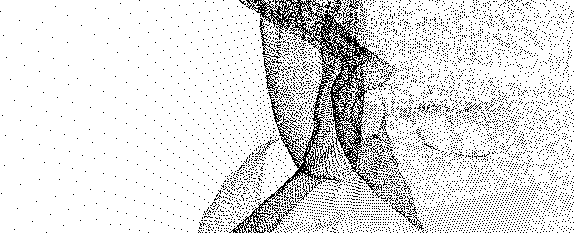
\includegraphics[width=7cm,frame]{random_weights_inv.png}
\caption{Weighted points downsampling using random weights}
\label{fig:random_weights}
\end{wrapfigure}
A simple way to distribute the weights is to set each weight to a random value. However, this leads to an irregular visual pattern in the way downsampled points are placed on the surfaces, as seen in figure \ref{fig:random_weights}. The left-hand side of the point cloud is not downsampled and retains the original regular pattern from the model.

\subsection{LOD regions}
Another possibility is to first compute several downsampled point sets $P'_{r}$ with fixed downsampling ratios $r$, during preprocessing. $P'$ is then produced out of pieces of these sets. The resulting $P'$ is thus composed of several \emph{level of detail} (LOD) regions\footnote{These are called \emph{mipmaps} in the implementation}, and so $\rho'(d)$ becomes a non-continuous staircase function, and visual discontinuities are produced. However, this method allows for producing the sets $P'_{r}$ without time constraints, and with a constant $r$.

In figure \ref{fig:uniform_example}, the region farther away was downsampled this way (using uniform downsampling). A visual discontinuity can be seen in the lower-right corner.

\subsection{Uniform downsampling}
Uniform downsampling is a downsampling algorithm that aims to produce a more regular pattern in the distribution of points on $P'$, as opposed to that produced by random downsampling (figure \ref{fig:random_weights}). It operates using a constant ratio $r$.

\begin{wrapfigure}{r}{7cm}
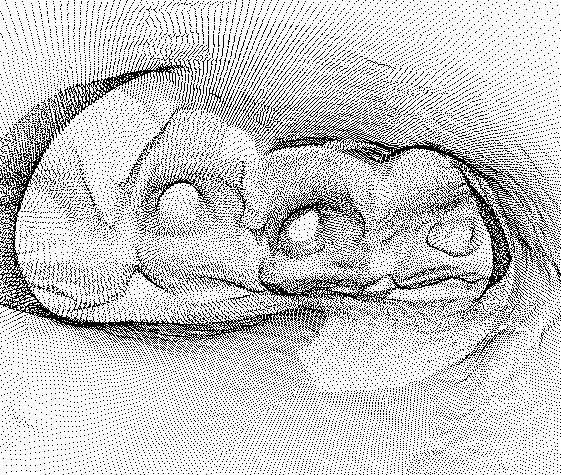
\includegraphics[width=7cm,frame]{uniform_example_inv.png}
\caption{Example of uniform downsampling}
\label{fig:uniform_example}
\end{wrapfigure}
The input point set $P$ is divided into a regular grid of cubes $C_{i,j,k}$ with side length $l$. For all cubes that contain at least one point, exactly one single point $p'$ is outputted into $P'$, whose position is the mean of that of the points in $C$, and whose color is that of the point $p \in P$ closest to that position. Figure \ref{fig:uniform_algo} illustrates the procedure in two dimensions. The more regular aspect of $P'$ is because its points are constrained by the regular grid. The algorithm also does not require $P$ to have a regular pattern to begin with.

The main difficulty is to find the value for the side length $l$, such that $n = |P'|$ is approximately equal to $r \times |P|$. Figure \ref{fig:uniform_stat} shows how $n$ varies in function of $l$ for some example models: In general, $n$ gets larger as the side length $l$ gets smaller, because there are more cubes available in the region of the model. Because the cubes are non-overlapping and each point $p \in P$ belongs to exactly one cube, $n$ is at most $|P|$. It reaches this value once $l$ reaches a value (depending on the density) where each point belongs to a different cube.

However, the function is not entirely monotonic, as the close-up view in figure \ref{fig:uniform_stat_detail} shows. This is because when $l$ gets changes, all cubes on the grid (except those at the origin) get displaced. So it is possible that two neighboring points fit into one cube for one value of $l$, but for $l' > l$ the grid becomes such that a boundary lies between these points. This effect only occurs at the small scale because as $l$ gets even larger, the boundary moves further so the two points again fit into one cube, and many more points in the model fit into the same cubes.

Because the points are not distributed evenly in space but rather on the object's surfaces, but the algorithm operates in three-dimensional space, there is no way to effectively estimate a value for $n(l)$. Instead the algorithm does a dichotomic search to find a value $l$ such that $n \approx r \times |P|$, within a certain tolerance. The small-scale ascending intervals of $l(n)$ are taken into account.

\begin{figure}[p]
\centering
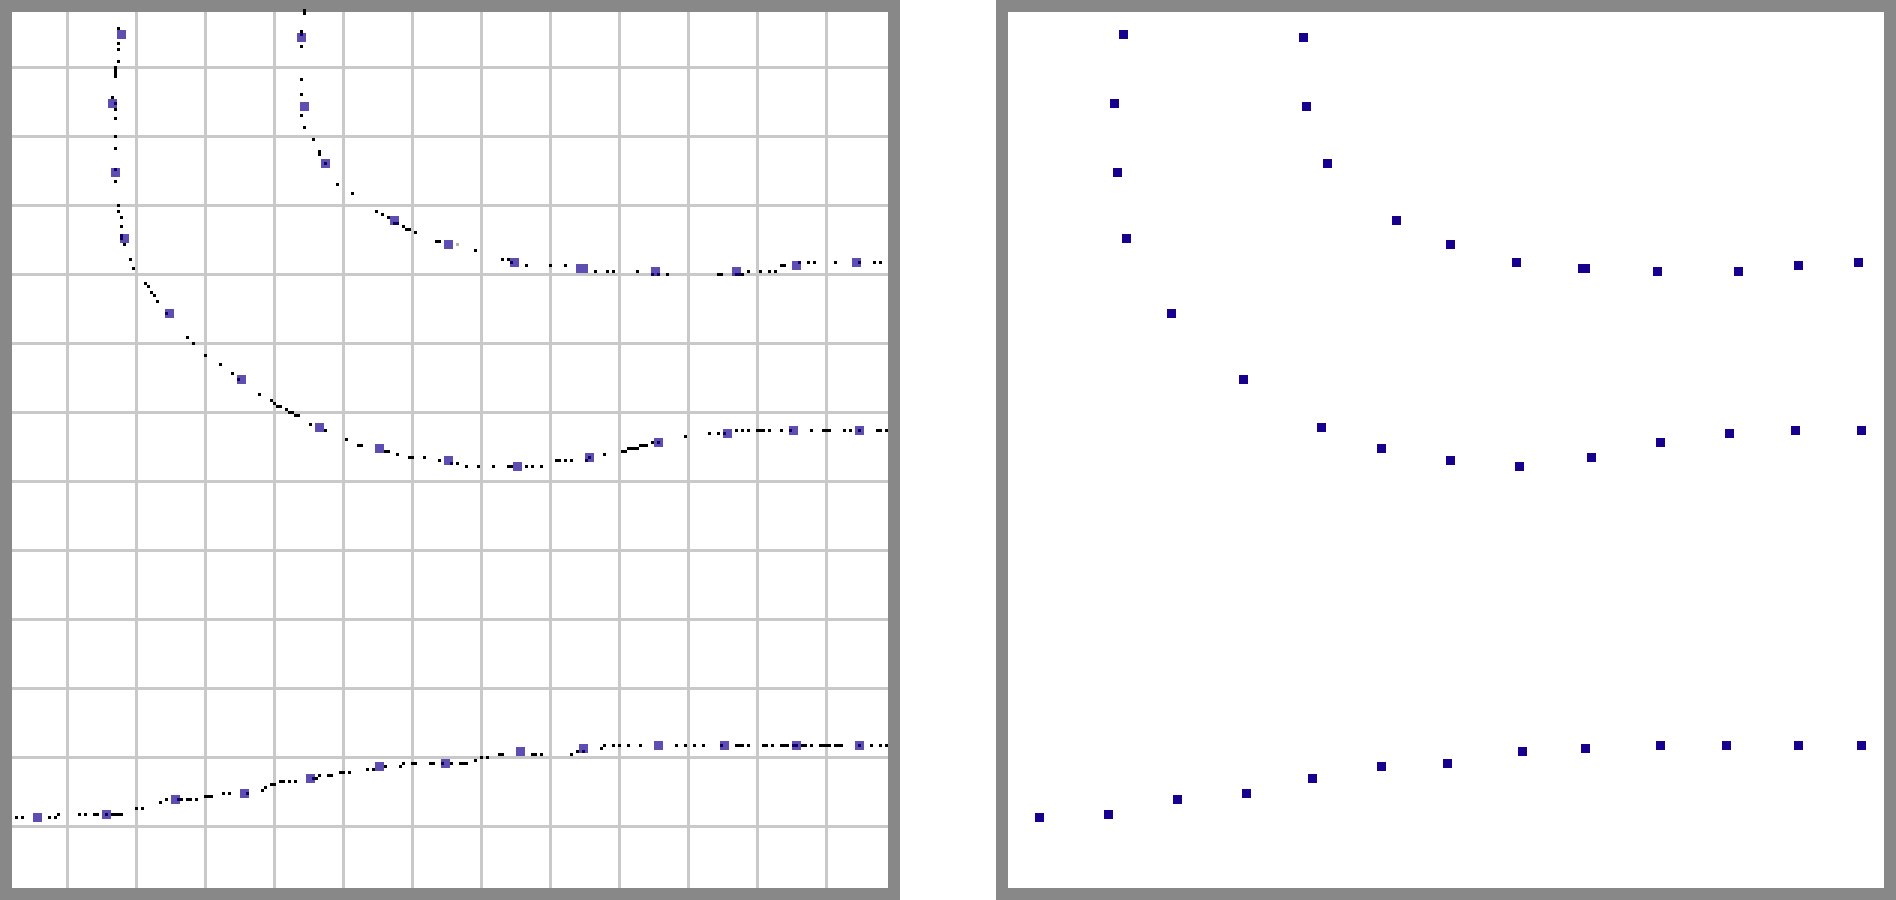
\includegraphics[width=7cm]{uniform.png}
\caption{Two-dimensional visualization of uniform downsampling algorithm}
\label{fig:uniform_algo}
\end{figure}

\begin{figure}[p]
\centering
\begin{gnuplot}
	set terminal epslatex color
	set xlabel "$l$"
	set ylabel "$n / |P|$"
	plot \
		"stat\_dragon.dat" using 1:($2/3609599+0*$2) smooth unique linetype rgb "black" title "dragon.ply", \
		"stat\_statuette.dat" using 1:($2/4999995+0*$2) smooth unique linetype rgb "red" title "statuette.ply", \
		"stat\_scan.dat" using 1:($2/681124+0*$2) smooth unique linetype rgb "blue" title "scan.ply"
\end{gnuplot}
\caption{Number of output points $n$ VS cubes side length $l$ in uniform downsampling}
\label{fig:uniform_stat}
\end{figure}

\begin{figure}[p]
\centering
\begin{gnuplot}
	unset key
	set ylabel "$n$"
	set xlabel "$s$"
	plot "uniform\_stat\_detail.dat" smooth unique
\end{gnuplot}
\caption{Close-up view of figure \ref{fig:uniform_stat}}
\label{fig:uniform_stat_detail}
\end{figure}


\subsection{Choosing the downsampling ratio}
The function $r(d)$ determines what ratio of downsampling that should be applied depending on the distance $d$ to the camera. If \emph{LOD regions} are used, it is a staircase function and can only take a small number of different values, otherwise (\emph{weighted points}) it is continuous. On what regions downsampling will be applied, and how $d$ is defined depends on the data structure used. (see next chapter.)

Let $L$ be the number of \emph{LOD regions} (``levels''). In the program, it is usually 1, 4, 8 or 16. For \emph{weighted points} downsampling, $L$ can take any value and can be changed at runtime. In both cases, $r(d)$ is defined the same way:

$r_{\ell}(\ell, a, L, n_{\text{total}}, n_{\min})$ gives the downsampling ratio for level $\ell \in [0, L-1]$. $n_{\text{total}}$ is the total number of points used as input to the downsampling algorithm, $n_{\min}$ the minimal number of points the should be outputted. If the algorithm is applied to the full model $n_{\text{total}} = |P|$ (number of points in model), and $n_{\min} = C$ (capacity of renderer) is used, since the goal is to stay as close as possible but inferior to $C$, so as to not lose more points than necessary. The function is defined such that $r_{\ell}(\ell = 0) = n_{\text{total}}$ (level 0 means no downsampling), $r_{\ell}(\ell = L-1) = n_{min}$ (maximal possible downsampling must be reached on last level), and it is stictly decreasing. The \emph{amount} parameter $a$ sets how strongly the function should be decreasing, and must be adjusted to fit the input model.

If \emph{LOD regions} are used, this function is evaluated during the preprocessing stage, when the $L-1$ downsampled point sets are created. For \emph{weighted points}, it is evaluated at runtime. Then, $a$ and $L$ also can be changed at runtime, and $\ell$ can take real values (as opposed to integers only). This allows for continuous downsampling.

The level to use at a given location is chosen by the function $\ell(d, s)$, where $d$ is the distance to the camera, and the \emph{setting} $s$ a parameter that can always be adjusted at runtime (unlike $a$). The function is defined such that $\ell(d = 0) = 0$ (no downsampling when very close to camera), and $\lim_{d \rightarrow \infty} = L-1$ (eventually reach maximal level). Also, it increases with $d$, where $s$ determines how quickly. $\ell(d, s)$ is defined as a real function, but when \emph{LOD regions} are used, the floor value $\lfloor \ell(d, s) \rfloor$ is always taken.

In short, the process of choosing the downsampling ratio $r(d)$ in function of distance $d$ works as follows: For \emph{weighted points}, $r(d) = r_{\ell}(\ell(d, s), a, L, n_{\text{total}}, n_{min})$ is evaluated at runtime, and $s, a, L$ can all be adjusted at runtime. Thus $r(d)$ is continuous.

For \emph{LOD regions}, $L$ point sets are created in the preprocessing stage which are downsampled with ratio $r_{ell}(i, a, L, n_{\text{total}}, n_{min})$. The integer $i \in 0 \hdots L-1$ is the level of the point set, and $a, L, n, n_{min}$ all need to be known in this stage. The program stores the downsampling ratios associated with the $L$ levels with the generated data structure. At runtime, the downsampled point set for level $i = \lfloor \ell(d, s) \rfloor$ is chosen depending on $d$. Only $s$ can be adjusted at runtime.

\subsection{Definition of the downsampling functions}
The downsampling level function $\ell$ is defined as follows:
\begin{displaymath}
	\ell(d, s) = \begin{cases}
		\min \{ \frac{d - d_{0}}{\Delta d}, L-1 \} & d > d_{0} \\
		0 & d \leq d_{0} \vee s = 0
	\end{cases}
\end{displaymath}

with $d_{0} = b^{1.3}$ the \emph{start distance}, i.e. the distance from the camera where downsampling should start, $\Delta d = b$ the \emph{step distance} after which the next level is chosen, and $b = \frac{250}{s}$.

So the level is chosen linearily with the distance, with an offset $d_{0}$. The \emph{setting} $s$ controls the intervals between levels and the start distance. The exponent $1.3$ for $d_{0}$ keeps $d_{0}$ larger than $\Delta d$, because the jump from no downsampling to the first level of downsampling represents a greater loss in output quality than a jump between downsampling levels.

The definition of $b$ makes sure $\ell(d)$ increases faster when $s$ is larger: If $s = 0$, $\ell$ is always zero, and no downsampling will be applied. If $d \gg 0$, eventually $\ell(d)$ will always yield the maximal downsampling level $L - 1$.

The following graph shows the function in its staircase form, with different values for $s$.

\begin{figure}[H]
\centering
\begin{gnuplot}
	set terminal epslatex color
	set ylabel "level"
	set xlabel "$d$"
	set ytics (0, 1, 2, 3, 4, 5, 6, 7, 8, 9, 10, 11, 12, 13, 14, 15)

	levels = 16
	xp = 1.3
	maxd = 700

	set xrange [0:maxd]
	set yrange [0:levels + 3]
	unset autoscale

	start_distance(b) = b**xp
	step_distance(b) = b
	constrain_lvl(l) = (l > levels - 1) ? (levels - 1) : l
	b(s) = 250 / s

	l(d, s) = constrain_lvl( \
		(d > start_distance(b(s))) ? ((d - start_distance(b(s))) / step_distance(b(s))) : 0 \
	)
	
	plot [d=0:maxd] \
		floor(l(d, 20)) with steps lt rgb "black" title "$s = 20$", \
		floor(l(d, 10)) with steps lt rgb "blue" title "$s = 10$", \
		floor(l(d, 50)) with steps lt rgb "red" title "$s = 50$"
\end{gnuplot}
\caption{Downsampling level for distance function $\ell(d, s)$}
\label{fig:downsampling_ell_d}
\end{figure}


The downsampling ratio function $r_{\ell}$ is defined as follows:
\begin{displaymath}
	r_{\ell}(\ell, a, L, n_{\text{total}}, n_{\min}) = 1 - (1 - r_{\min}) \left( \frac{\ell}{L-1} \right)^{a}
\end{displaymath}
where $r_{min} = \max \{ \frac{n_{\min}}{n_{\text{total}}}, 1 \}$ is the minimal downsampling ratio. Note that when $n_{\text{total}} \leq n_{min}$, the function always yields $1$ and no downsampling will be applied. 

The following graph shows the function with different values for the downsampling amount $a$:

\begin{figure}[H]
\centering
\begin{gnuplot}
	set terminal epslatex color
	set ylabel "$r$"
	set xlabel "level"
	set xtics (0, 1, 2, 3, 4, 5, 6, 7, 8, 9, 10, 11, 12, 13, 14, 15)

	n = 5000000
	nmin = 1000000
	rmin = nmin / n
	levels = 16

	set xrange [0:(levels - 1)]
	set yrange [0:1]
	unset autoscale
	
	r(l, a) = 1 - (1 - rmin) * (l/(levels - 1))**a
	plot [l=0:(levels - 1)] \
		r(l, 2) lt rgb "black" title "$a = 2.0$", \
		r(l, 1.2) lt rgb "blue" title "$a = 1.2$", \
		r(l, 0.4) lt rgb "green" title "$a = 0.4$", \
		r(l, 3.8) lt rgb "red" title "$a = 3.8$"
\end{gnuplot}
\caption{Downsampling ratio function $r_{\ell}(d, a)$}
\label{fig:downsampling_r_ell}
\end{figure}

\begin{wrapfigure}{r}{7cm}
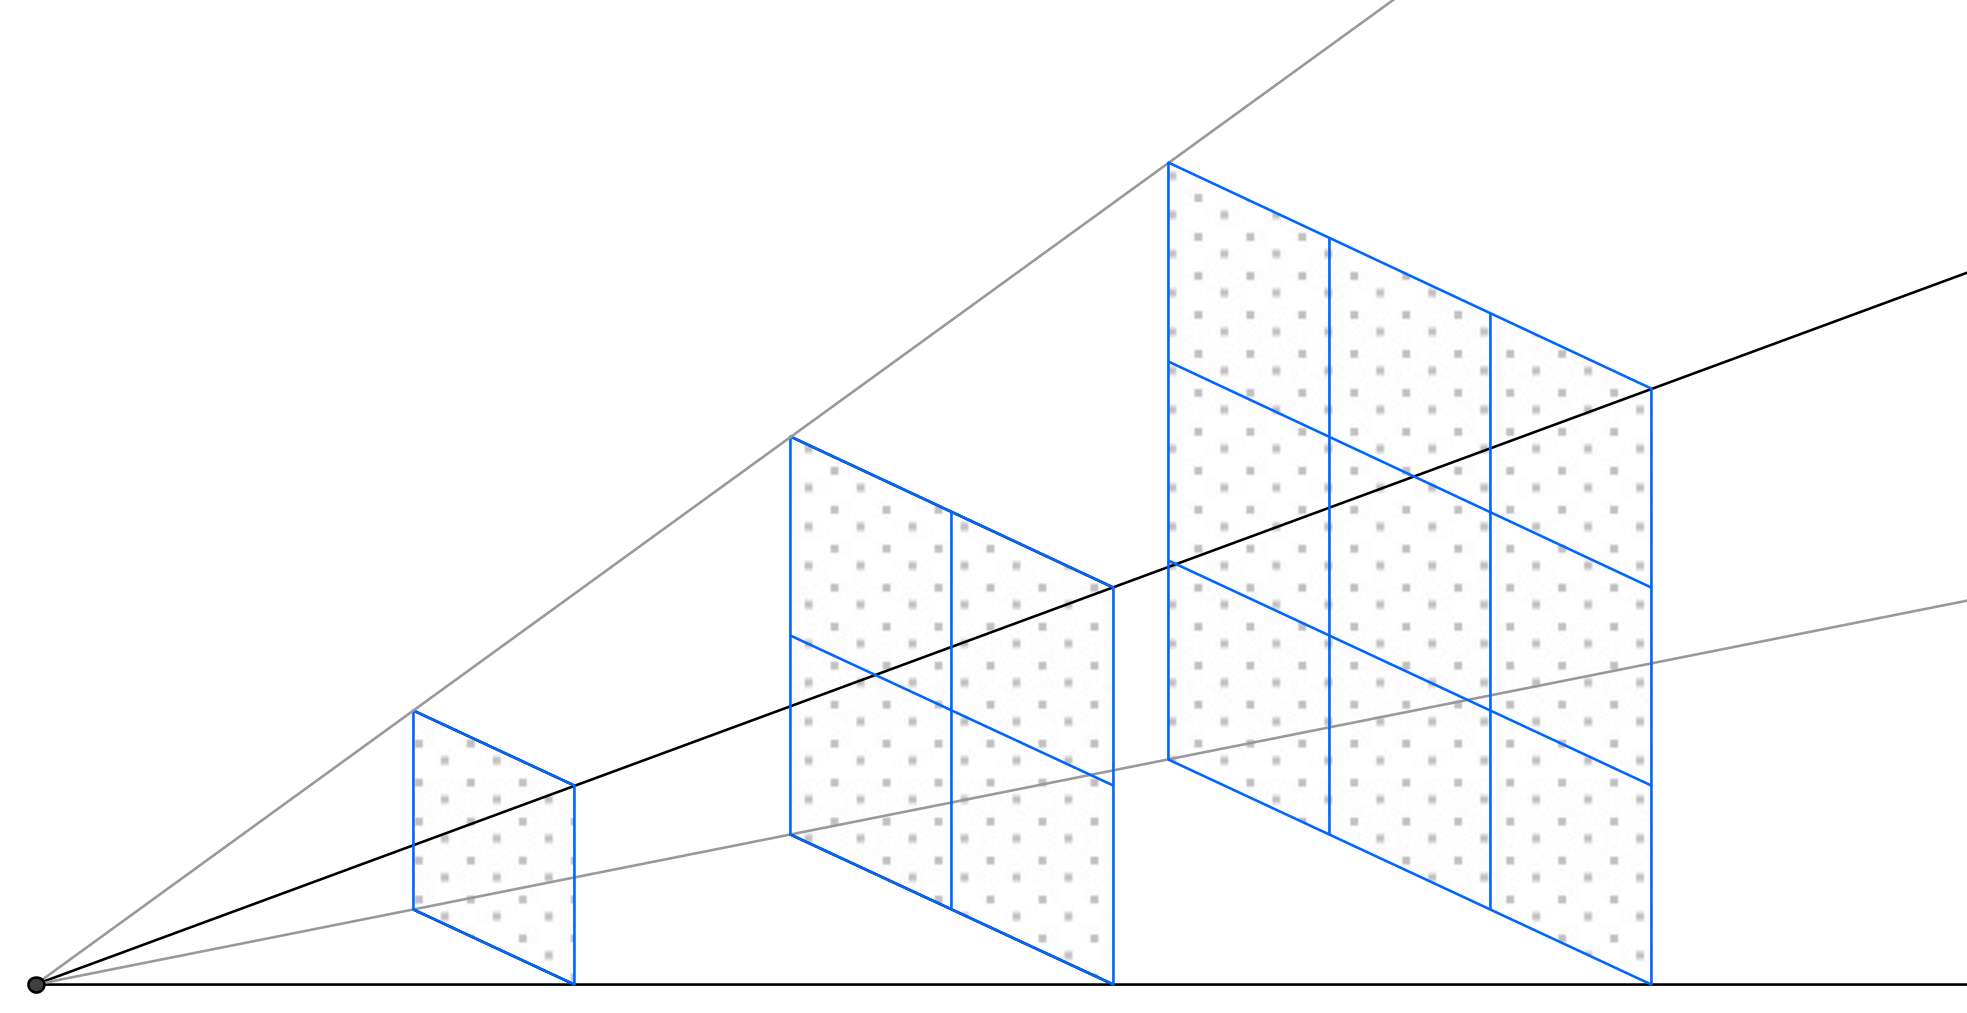
\includegraphics[width=7cm]{distanceDensity.png}
\caption{Perspective projection and area}
\label{fig:distance_density}
\end{wrapfigure}
Figure \ref{fig:distance_density} shows visible areas\footnote{In reality, the areas would be curved (intersection of view frustum and sphere of radius $d$), but the simplification holds because the field of view is small} with distances $d$, $2d$ and $3d$ to the camera in a perspective projection. Their area is proportional to $d^{2}$. Supposing that surfaces of the point cloud is located exactly on these areas, the point density of the projection $\rho'$ would also be proportional to $d^{2}$.

Since $\rho'$ should be more or less constant, setting $a = 2$ makes sense as it cancels out the effect. In practice, it needs to be adjusted to fit the particular point cloud.

Finally, this graph shows $r_{d, s}$ ($r_{\ell} \circ \ell$) in piecewise form, with $a = 2$, $L = 16$ and $r_{\min} = 0.2$:

\begin{figure}[H]
\centering
\begin{gnuplot}
	set terminal epslatex color
	set ylabel "$r$"
	set xlabel "$d$"

	levels = 16
	xp = 1.3
	maxd = 800
	n = 5000000
	nmin = 1000000
	rmin = nmin / n
	a = 2
	b(s) = 250 / s

	start_distance(s) = b(s)**xp
	step_distance(s) = b(s)
	constrain_lvl(l) = (l > levels - 1) ? (levels - 1) : l

	r(l) = 1 - (1 - rmin) * (l/(levels - 1))**a

	l(d, s) = constrain_lvl( \
		(d > start_distance(s)) ? ((d - start_distance(s)) / step_distance(s)) : 0 \
	)
	
	rd(d, s) = r( 0.0 + floor( l(d, s) ) )
	rdc(d, s) = r( 0.0 + l(d, s) )
	
	plot [d=0:maxd] \
		rd(d, 20) with steps lt rgb "black" title "$s = 20$", \
		rd(d, 10) with steps lt rgb "blue" title "$s = 10$", \
		rd(d, 50) with steps lt rgb "red" title "$s = 50$"
\end{gnuplot}
\caption{Downsampling ratio for distance $r(d, s)$}
\label{fig:downsampling_r}
\end{figure}

\subsection{Adaptive downsampling}

\begin{figure}[p]
\centering
\begin{gnuplot}
	set terminal epslatex color
	set xlabel "$s$"
	set ylabel "$|P'| / n_{\min}$"
	set yrange [0.0:1.1]

	nmin = 1000000
	plot \
		"setting\_output\_stat/statuette\_inside\_cm8.dat" using 1:($2/nmin+0*$2) smooth unique title "statuette inside cm8", \
		"setting\_output\_stat/statuette\_far\_cm8.dat" using 1:($2/nmin+0*$2) smooth unique title "statuette far cm8", \
		"setting\_output\_stat/dragon\_inside\_cm8.dat" using 1:($2/nmin+0*$2) smooth unique title "dragon inside cm8", \
		"setting\_output\_stat/dragon\_inside\_c.dat" using 1:($2/nmin+0*$2) smooth unique title "dragon inside c", \
		"setting\_output\_stat/dragon\_closeup\_cm8.dat" using 1:($2/nmin+0*$2) smooth unique title "dragon closeup cm8"
\end{gnuplot}
\caption{Number of output points $n$ VS cubes side length $s$ in uniform downsampling; normalized by number of points in model $|P|$}
\label{fig:uniform_stat}
\end{figure}


\section{Occlusion culling}


\chapter{Data structures}
The $f_{P}$ function described in the previous chapter takes a unordered set $P$ of three-dimensional points as input. In an implementation, $P$ will be stored in a certain \emph{data structure}, which is essentially a way of representing $P$ using a one-dimensional array of bits. The data structure will hold the points $P$, along with weights or LOD sets for downsampling, and possibly additional information. The criterion for choosing a data structure is that $f_{P}$ can be implemented in an efficient way.

\section{General}
Since the data structure must contain all the $n_{\text{total}}$ points of $P$, its size must always be at least in $O(n_{\text{total}})$. The algorithm which extracts $P' = f_{P}$ will typically only need to read a small portion consisting of $n \ll n_{\text{total}}$ points. To make this efficient the data structure must be designed such that:
\begin{itemize}
\item It must be possible to determine the portions of data to extract without searching through the whole structure. The worst case would be a data structure that consists simply of an array of points in any order, because in order to find the points that lie inside the current view frustum the algorithm would have to check every point in the array, leading to a time complexity $O(n_{\text{total}})$. This would defeat the goal of enabling efficient loading of large models.
\item The data structure is always serialized to storage in one dimension. It is generally much more efficient to read a small number of long segments, rather than many small segments: Seeking times on the storage device are avoided, and various caching mechanisms from the underlying file system are used.

No order can be defined for three dimensional points, but their one-dimensional representations always have an order. So a compromise needs to be found by which the serialization is ordered such that for the majority of cases, points that are close to each other in three dimensional space remain close to each other in the serialization.
\end{itemize}

Two techniques are used to achieve this: The model is split into smaller \emph{regions}, and the points within that region remain grouped together in the data structure. Points within the same regions have the property that their distance is upper bounded by the size of the region, and so this contributes to the ordering issue. Also, \emph{pointers} is used in various ways, meaning reading algorithm will directly jump to a given offset in the data independently of its distance.

\section{File types}
The data structure is built on top of a \emph{file type}. Several possible file types were compared:
\begin{description}
\item[Raw file] Essentially no file type is used, and the data structure is implemented on the lowest level. The implementation needs to write and read the structure as a single continguous segment of binary data. This allows for the highest level of control, but requires an ad-hoc definition of helper structures such as a way to split the file into different parts for points, downsampled points, regions, additional file information... Also the precise way that data values serialized (floating point and integer data types, alignment, endianess) needs to be taken care of in the implementation of the data structure.
\item[ASCII-based file] Storing data as an ASCII-based text file instead of as raw binary data removes the latter problems of data serialization. The remaining problems stay the same. The files get much larger: If the file contains a set of $1000000$ points with $x, y, z$ coordinates, storing them as 4 byte floating point values would require $\SI{11. 72}{\mega\byte}$. If the values are written in decimal representation with 8 digits, plus separation characters, a size of about $\SI{29. 56}{\mega\byte}$ would result. This additional space requirement, and the parsing overhead when reading from the file, makes such file types impractical for large amounts of data.
\item[XML] XML would provide a way to represent structured data, and so it would be possible to build the data structure in terms of XML tags, containers and attributes. However, it suffers the same problems as any ASCII-based format, to an increased extent since it tends to be very verbose compared to simpler formats. Also, the purpose of XML is not to deal with large amounts of data that is dynamically read, but rather to deal with relatively small, deeply structured files such as computer programs or web pages, and it provides tools to validate, transform, interlink, etc. such files.
\item[HDF] HDF (\emph{Hierarchical Data Format}) is the main format used in the program. It is a binary designed designed for storage of large quantities or scientific data in such a way that parts of it can be extracted efficiently. It allows for the definition of simple or combound data types (such as 3 floating point values and 3 bytes for an XYZRGB point), and can store several data sets or such values in the file. These data sets are ordered arrays of one or more dimensions, and the \emph{hyperslap} mechanism provides a way to efficiently read or write in it. HDF stores the data sets either directly as sequential data on the storage device, but can also internally store the data sets in multiple chunks, and provide additional optimizations such as internal caches for dealing with large data sets.
\item[SQL database] 
\end{description}

\section{Cuboid regions} \label{sec:cub_reg}
All of the data structures used in the projet rely on subdividing the three dimensional space in axis-aligned cuboid regions. A cuboid $\mathcal{C}$ is defined by its \emph{origin} $(x, y, z)$ and its \emph{extremity} $(x', y', z')$, and a point $\overrightarrow{p}$ is considered to be inside the cuboid if and only if $p_{x} \in [x, x'[$, $p_{y} \in [y, y'[$ and $p_{z} \in [z, z'[$.

Because the intervals are open on one side, points that lie on the border of two adjacent cuboid can never fall into both cuboids. However, when defining a bounding cuboid that should enclose a given set of points, it becomes necessary to make the coordinates of its extremity slighly larger than the point with maximal coordinates.

\subsection{Floating point issues}
Cuboids are defined in terms of origin and extremity, instead of origin and side lengths, in order to deal with floating point imprecision problems that would otherwise occur in the implementation: For the \emph{tree structures}, cuboids will be recursively subdivided into smaller cuboids, out of which some share extremitiy coordinates with the parent cuboid. If side length were to be used, those floating point values would not be copied, but rather need to be recomputed from the new origins and side lengths of the child cuboids. This could make their values slightly different, and as a consequence the algorithms would be incorrect, as they could for instance encounter points that are inside a child cuboid, but outside the parent cuboid.
These edge cases are significant because the coordinates are real values, whereas quantities of points are discrete. Parts of the program rely on having exact knowledge of these quantities, for example to align data segments in files the right way.

In other situations where floating point imprecisions are tolerated, the program uses a small threshold value $\epsilon$ to test two floating point values for ``equality''. That is, $f_{1} \approx f_{2} \Longleftrightarrow |f_{1} - f_{2}| < \epsilon$.

\subsection{Point-to-cuboid distance}
Also for all of the data structures, the implementation of $f_{P}$ will apply downsampling to entire cuboid regions with a constant downsampling ration $r$. This ratio is determined by $r(d, s)$ as described in the previous chapter, where $d(\overrightarrow{p}, \mathcal{C})$ is a \emph{point-to-cuboid distance} from the camera position to the cuboid. The program allows the user to choose between several definitions for $d$:
\begin{description}
\item[center] The distance from $\overrightarrow{p}$ to the centroid $( \frac{x + x'}{2}, \frac{y + y'}{2}, \frac{z + z'}{2} )$ of $\mathcal{C}$.
\item[minimal] The minimal distance from $\overrightarrow{p}$ to any position $\overrightarrow{q}$ on the border of $\mathcal{C}$. The $\overrightarrow{q}$ which gives the minimal distance may be a corner of $\mathcal{C}$, or an orthogonal projection of $\overrightarrow{p}$ on either an edge or a side of $\mathcal{C}$.
\item[maximal] The maximal distance from $\overrightarrow{p}$ to any position $\overrightarrow{q}$ on the border of $\mathcal{C}$. In this case, $\overrightarrow{q}$ is always a corner of $\mathcal{C}$.
\item[mean] The mean value of the minimal and maximal distances.
\end{description}

\begin{wrapfigure}{r}{4cm}
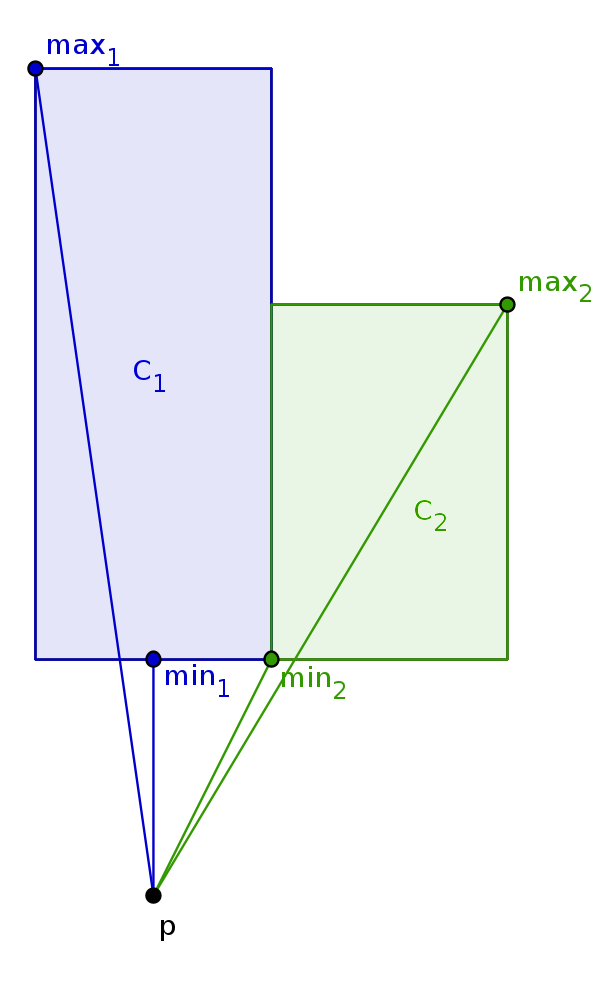
\includegraphics[width=4cm]{minMaxDistance.png}
\label{fig:min_max_c_d}
\end{wrapfigure}
Assuming that any definition of $d$ gives a value $\geq$ the maximal distance and $\leq$ the minimal distance, it is not possible in general to define $d$ such that if $d(\overrightarrow{p}, \mathcal{C_{1}}) > d(\overrightarrow{p}, \mathcal{C_{2}})$, then for all $\overrightarrow{q_{1}} \in \mathcal{C_{1}}$ and all $\overrightarrow{q_{2}} \in \mathcal{C_{2}}$, it remains true that $d(\overrightarrow{p}, \overrightarrow{q_{1}}) > d(\overrightarrow{p}, \overrightarrow{q_{2}})$. 

The figure on the right illustrates this: $d(p, \min_{1}) < d(p, \min_{2})$, whereas $d(p, \max_{1}) > d(p, \max_{2})$. So no matter how the \emph{point-to-cuboid distance} is defined in that case, there will always be points in one of the cuboids that don't fullfill the condition. When such points are inside the view frustum, is leads to visual discontinuities, as there are places where the downsampling ratio gets lower at a greater distance instead of higher.

As a compromise, one of the proposed definitions needs to be chosen chosen that reduces this effect. Generally, better results are produces when the regions are more or less cubic, and in that case the \textbf{center} definition of $d$ yields good results. Otherwise, \textbf{minimal} tends to be better.

\pagebreak

\section{Cubes structure}
The \emph{cubes structure} is a first attempt at a simple way to organize the set of points such that the algorithm is faster than a naive implementation which would iterate through the whole set of points at each evaluation of $f_{P}$.

Space is subdivided into a regular grid of axis-aligned \emph{cubes} $\mathcal{C}_{i,j,k}$ with a common side length $l$.\footnote{This is unrelated to the cubes used for uniform downsampling in the previous chapter.} These cubes are the cuboid regions for this structure. Because of the way their boundaries are defined, every point $p \in P$ will belong into exactly one cube. The side length can be configured when the structure is created, and is by default set to $l = 5$. $i, j, k$ are the coordinates for the cubes in the grid. For the cube $\mathcal{C}_{0,0,0}$, its \emph{origin} corresponds to the origin of the space.

Only cubes that contain at least one point are created, so their total number will be finite. In the first stage of the structure creation progress, the algorithm iterates through the full set of points $P$, for each point $p$ and determines the coordinates of the cube into $p$ will belong by floor division:
\begin{equation*}
	(i, j, k) = \left( \lfloor p_{x}/l \rfloor, \lfloor p_{y}/l \rfloor, \lfloor p_{z}/l \rfloor \right)
\end{equation*}
This is correct because the definition of the floor function coincides with the way that the cuboid regions' boundary intervals are defined. Similar relations will occur for the tree structures, where it is critical for the correct functionning of the algorithm that the relations always hold, despite possible floating point imprecision errors.

There are two variants for the cubes structure, one with \emph{weighted points} and one with \emph{LOD regions}. For the weighted points variant, the algorithm proceeds by attributing random weights $w \in [0,1]$ to each point $p \in P$ in an uniform distribution. For the LOD regions variant, the algorithm instead computes for each cube $\mathcal{C}$, the $L-1$ downsampled point sets, for the set of points inside that cube $P(\mathcal{C}) = \{ p \mid p \in \mathcal{C} \}$.

\subsection{Serialization}
There are two implementations of the cubes structure: Using \emph{HDF} as file type, and using an \emph{SQLite database}. For the \emph{HDF} file, the points are stored into a data set, and are ordered such that points belonging to the same cube are grouped. The order of the groups and the order of the points within the groups does not make a difference. The combound type for this data set consists of 3 floating point values for the $x, y, z$ coordinates of the point, and 3 byte values for the color values.

\section{Tree structures}
\subsection{Octree}
\subsection{KdTree}

\chapter{Implementation}

\chapter{Results}

\chapter{Conclusion}

\appendix
\chapter{Geometry algorithms}

\section{Definitions}
The geometric objects used in the algorithms are defined in the following manner:
\begin{description}
\item[cuboid] Axis-aligned cuboid $\mathcal{C}$ is defined by \emph{origin} point $x, y, z$, and \emph{extremity} point $x', y', z'$, such that $x' > x$, $y' > y$ and $z' > z$. The coordinate intervals are open on the extremity side, i.e. a point $\overrightarrow{p}$ is considered to be inside the cuboid if and only if $p_{x} \in [x, x'[$, $p_{y} \in [y, y'[$ and $p_{z} \in [z, z'[$. See section \ref{sec:cub_reg} for further explanation.

\item[plane] An oriented two-dimensional plane $P$ in three-dimensional space is defined using four real values $a, b, c, d$. $\overrightarrow{n} = (a, b, c)$ is a normal vector of the plane, while $d$ is the distance from the origin to the plane, multiplied by $|\overrightarrow{n}|$.

In its \emph{normalized} form, $a, b, c, d$ are defined such that $|\overrightarrow{n}| = 1$. Then $d$ is simply the distance from the origin to the plane, and each plane there is exactly one normalized form.

The planes are oriented, that is an (oriented) distance from a point $\overrightarrow{p}$ to the plane is positive when $\overrightarrow{n} \cdot \overrightarrow{p} \geq 0$, and negative otherwise.

\item[frustum] A frustum is defined using the 6 planes that delimit it: the near, far, left, right, top and bottom planes. Supposing that the normal vectors of the planes are all pointing inside the frustum, a point is considered to be inside the frustum if and only if its oriented distance to each one of the planes of positive.

This representation of a frustum not unique, and is only valid when the 6 planes are arranged so as to delimit a frustum. A frustum can be defined using a 4x4 projection matrix, and the following algorithm describes how to get the 6 planes out of it.
\end{description}

\section{Projection matrix to view frustum} \label{frustum_planes}
Let $\matrixsym{M}$ be a projection matrix, and $\matrixsym{M}[i, j]$ be the value in $\matrixsym{M}$ at column $i$ and row $j$, counting from 0.
As described in \cite{Gri2001}, the 6 planes $P = (a, b, c, d)$ can be derived as follows:
\begin{align*}
	P_{\text{near}}   = (\matrixsym{M}[0, 3] + \matrixsym{M}[0, 2], \quad \matrixsym{M}[1, 3] + \matrixsym{M}[1, 2], \quad \matrixsym{M}[2, 3] + \matrixsym{M}[2, 2], \quad \matrixsym{M}[3, 3] + \matrixsym{M}[3, 2]) \\
	P_{\text{far}}    = (\matrixsym{M}[0, 3] - \matrixsym{M}[0, 2], \quad \matrixsym{M}[1, 3] - \matrixsym{M}[1, 2], \quad \matrixsym{M}[2, 3] - \matrixsym{M}[2, 2], \quad \matrixsym{M}[3, 3] - \matrixsym{M}[3, 2]) \\
	P_{\text{left}}   = (\matrixsym{M}[0, 3] + \matrixsym{M}[0, 0], \quad \matrixsym{M}[1, 3] + \matrixsym{M}[1, 0], \quad \matrixsym{M}[2, 3] + \matrixsym{M}[2, 0], \quad \matrixsym{M}[3, 3] + \matrixsym{M}[3, 0]) \\
	P_{\text{right}}  = (\matrixsym{M}[0, 3] - \matrixsym{M}[0, 0], \quad \matrixsym{M}[1, 3] - \matrixsym{M}[1, 0], \quad \matrixsym{M}[2, 3] - \matrixsym{M}[2, 0], \quad \matrixsym{M}[3, 3] - \matrixsym{M}[3, 0]) \\
	P_{\text{bottom}} = (\matrixsym{M}[0, 1] + \matrixsym{M}[0, 1], \quad \matrixsym{M}[1, 3] + \matrixsym{M}[1, 1], \quad \matrixsym{M}[2, 3] + \matrixsym{M}[2, 1], \quad \matrixsym{M}[3, 3] + \matrixsym{M}[3, 1]) \\
	P_{\text{top}}    = (\matrixsym{M}[0, 1] - \matrixsym{M}[0, 1], \quad \matrixsym{M}[1, 3] - \matrixsym{M}[1, 1], \quad \matrixsym{M}[2, 3] - \matrixsym{M}[2, 1], \quad \matrixsym{M}[3, 3] - \matrixsym{M}[3, 1])
\end{align*}

\section{Maximal point-to-cuboid distance}
The maximal distance from a point $\overrightarrow{p}$ to a cuboid $\mathcal{C}$ is always the distance to one of the 8 corners of $\mathcal{C}$. The algorithm simply tests the distances from $\overrightarrow{p}$ to each one of the corners and returns the maximal one. As a small optimization, the algorithm can compare the squares of the distances instead, so as to do only one square root computation.

\section{Minimal point-to-cuboid distance}

\section{Frustum-cuboid intersection}

\bibliographystyle{plain}
\bibliography{report}


\end{document}
